% -*-latex-*-
% 
% For questions, comments, concerns or complaints:
% thesis@mit.edu
% 
%
% $Log: cover.tex,v $
% Revision 1.8  2008/05/13 15:02:15  jdreed
% Degree month is June, not May.  Added note about prevdegrees.
% Arthur Smith's title updated
%
% Revision 1.7  2001/02/08 18:53:16  boojum
% changed some \newpages to \cleardoublepages
%
% Revision 1.6  1999/10/21 14:49:31  boojum
% changed comment referring to documentstyle
%
% Revision 1.5  1999/10/21 14:39:04  boojum
% *** empty log message ***
%
% Revision 1.4  1997/04/18  17:54:10  othomas
% added page numbers on abstract and cover, and made 1 abstract
% page the default rather than 2.  (anne hunter tells me this
% is the new institute standard.)
%
% Revision 1.4  1997/04/18  17:54:10  othomas
% added page numbers on abstract and cover, and made 1 abstract
% page the default rather than 2.  (anne hunter tells me this
% is the new institute standard.)
%
% Revision 1.3  93/05/17  17:06:29  starflt
% Added acknowledgements section (suggested by tompalka)
% 
% Revision 1.2  92/04/22  13:13:13  epeisach
% Fixes for 1991 course 6 requirements
% Phrase "and to grant others the right to do so" has been added to 
% permission clause
% Second copy of abstract is not counted as separate pages so numbering works
% out
% 
% Revision 1.1  92/04/22  13:08:20  epeisach

% NOTE:
% These templates make an effort to conform to the MIT Thesis specifications,
% however the specifications can change.  We recommend that you verify the
% layout of your title page with your thesis advisor and/or the MIT 
% Libraries before printing your final copy.

\title{Trychtýřová anténa s dielektrickou čočkou realizovaná technologií 3D tisku}

\author{Michal Průša}
% If you wish to list your previous degrees on the cover page, use the 
% previous degrees command:
%       \prevdegrees{A.A., Harvard University (1985)}
% You can use the \\ command to list multiple previous degrees
%       \prevdegrees{B.S., University of California (1978) \\
%                    S.M., Massachusetts Institute of Technology (1981)}
\department{katedra elektromagnetického pole}

\Work{Diplomová práce}
\WORK{DIPLOMOVÁ PRÁCE}

\FACULTY{FAKULTA ELEKTROTECHNICKÁ}
\faculty{fakulta elektrotechnická}
%\faculty{fakulta elektrotechnická}
% If the thesis is for two degrees simultaneously, list them both
% separated by \and like this:
% \degree{Doctor of Philosophy \and Master of Science}
\degree{Bakalar}

% As of the 2007-08 academic year, valid degree months are September, 
% February, or June.  The default is June.
\degreemonth{Květen}
\degreeyear{2017}
\thesisdate{May 20, 2017}

%% By default, the thesis will be copyrighted to MIT.  If you need to copyright
%% the thesis to yourself, just specify the `vi' documentclass option.  If for
%% some reason you want to exactly specify the copyright notice text, you can
%% use the \copyrightnoticetext command.  
%\copyrightnoticetext{\copyright IBM, 1990.  Do not open till Xmas.}

% If there is more than one supervisor, use the \supervisor command
% once for each.
\supervisor{Ing. Tomáš Kořínek PhD.}
% This is the department committee chairman, not the thesis committee
% chairman.  You should replace this with your Department's Committee
% Chairman.
\chairman{Arthur C. Smith}{Chairman, Department Committee on Graduate Theses}

% Make the titlepage based on the above information.  If you need
% something special and can't use the standard form, you can specify
% the exact text of the titlepage yourself.  Put it in a titlepage
% environment and leave blank lines where you want vertical space.
% The spaces will be adjusted to fill the entire page.  The dotted

\makecover
% lines for the signatures are made with the \signature command.

\thispagestyle{empty}
\null\newpage
\maketitle

\cleardoublepage
\thispagestyle{empty}
\section*{Čestné prohlášení}

% $Log: abstract.tex,v $
% Revision 1.1  93/05/14  14:56:25  starflt
% Initial revision
% 
% Revision 1.1  90/05/04  10:41:01  lwvanels
% Initial revision
% 
%
%% The text of your abstract and nothing else (other than comments) goes here.
%% It will be single-spaced and the rest of the text that is supposed to go on
%% the abstract page will be generated by the abstractpage environment.  This
%% file should be \input (not \include 'd) from cover.tex.
Prohlašuji, že jsem zadanou bakalářskou práci „Trychtýřová anténa s dielektrickou čočkou realizovaná technologií 3D tisku“ zpracoval sám s přispěním vedoucího práce a používal jsem pouze literaturu uvedenou na konci práce. Souhlasím se zapůjčováním práce a jejím zveřejňováním.
\vspace{2cm}

\noindent V Praze dne 18.5.2017 \hfill Michal Průša


\cleardoublepage

% $Log: abstract.tex,v $
% Revision 1.1  93/05/14  14:56:25  starflt
% Initial revision
% 
% Revision 1.1  90/05/04  10:41:01  lwvanels
% Initial revision
% 
%
%% The text of your abstract and nothing else (other than comments) goes here.
%% It will be single-spaced and the rest of the text that is supposed to go on
%% the abstract page will be generated by the abstractpage environment.  This
%% file should be \input (not \include 'd) from cover.tex.

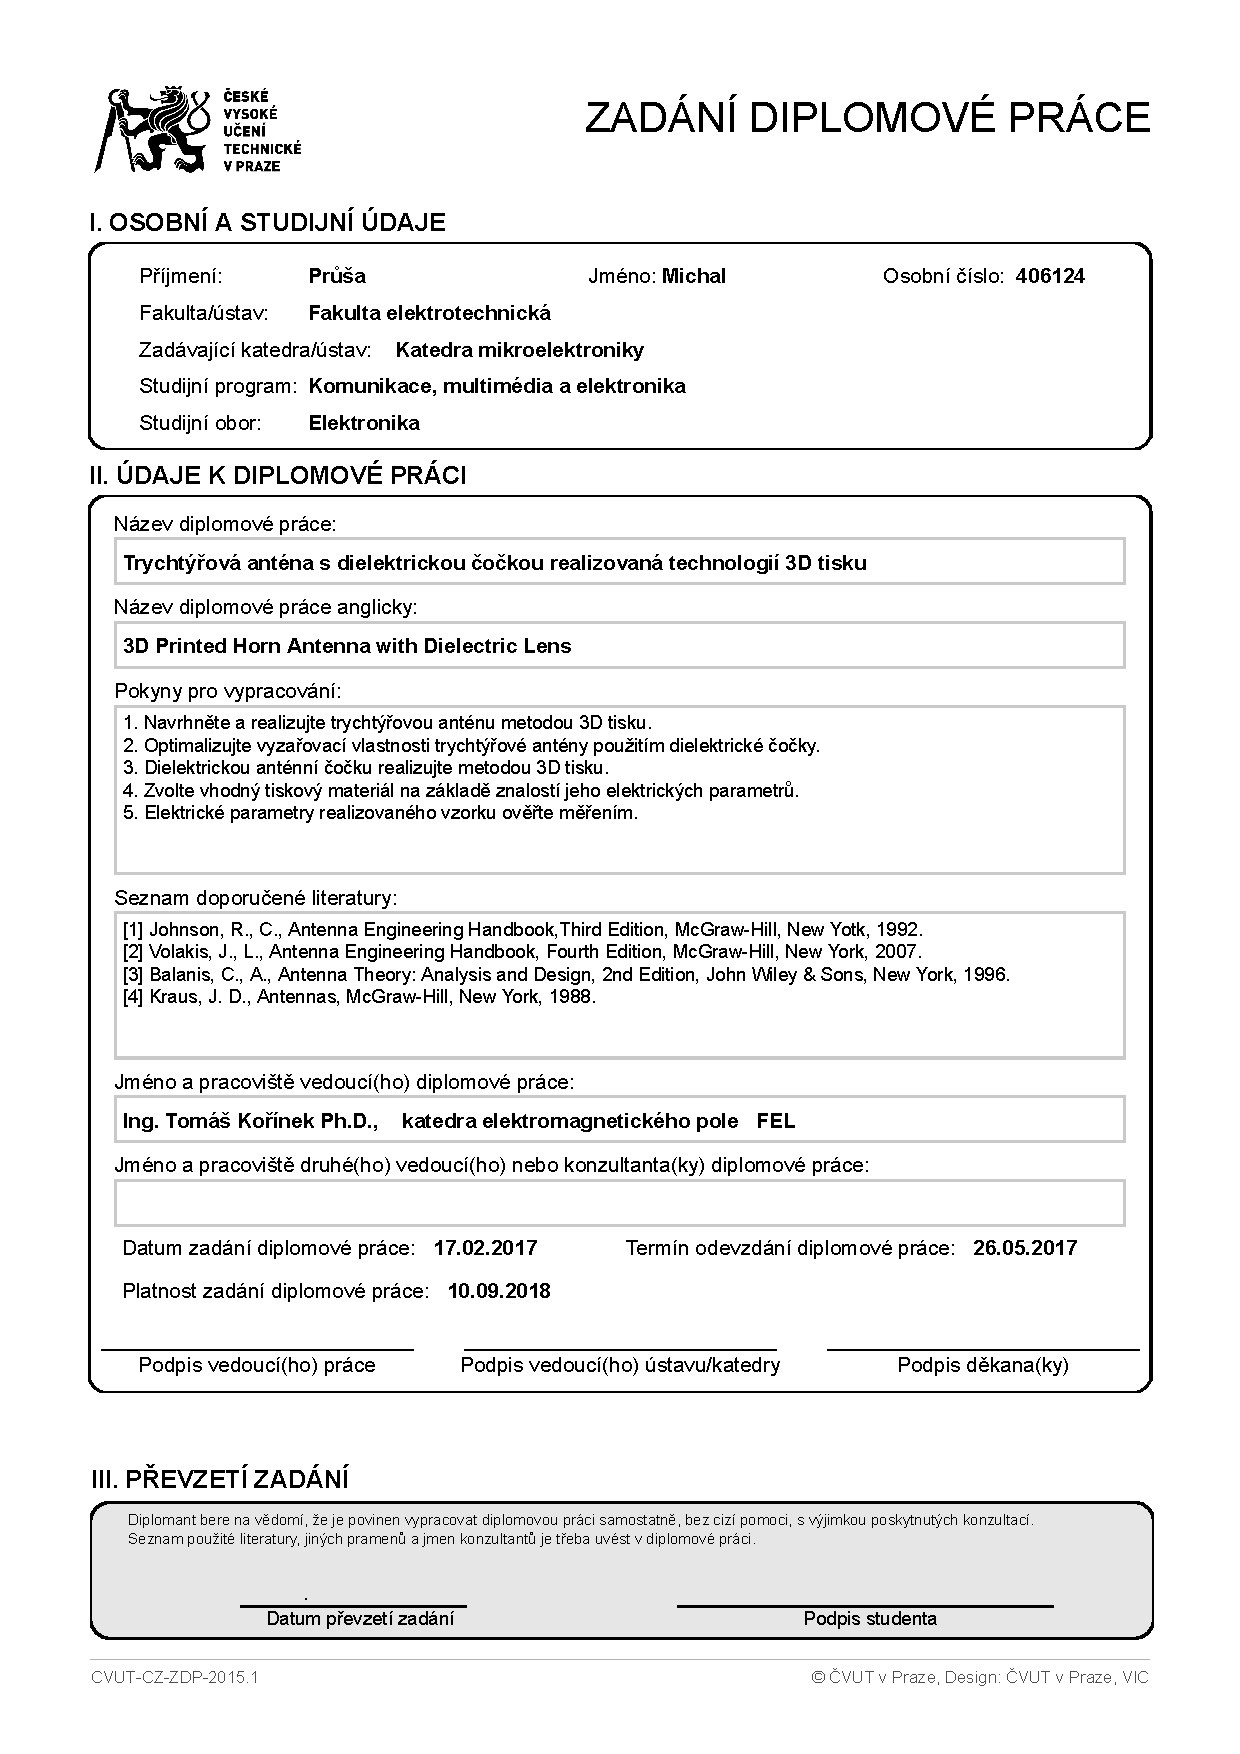
\includepdf[pages={1}]{zadani-nosign.pdf}


\cleardoublepage


\cleardoublepage
\thispagestyle{empty}
\section*{Poděkování}

% $Log: abstract.tex,v $
% Revision 1.1  93/05/14  14:56:25  starflt
% Initial revision
% 
% Revision 1.1  90/05/04  10:41:01  lwvanels
% Initial revision
% 
%
%% The text of your abstract and nothing else (other than comments) goes here.
%% It will be single-spaced and the rest of the text that is supposed to go on
%% the abstract page will be generated by the abstractpage environment.  This
%% file should be \input (not \include 'd) from cover.tex.
Mé poděkování patří panu Ing. Tomášovi Kořínkovi PhD. za cenné rady při konzultacích, za podporu, ochotu, vstřícnost a trpělivost při vedení celé této diplomové práce.

Dále mé poděkování patří firmě Prusa Research s.r.o. za poskytnutí tiskové laboratoře a finančních prostředků.


% The abstractpage environment sets up everything on the page except
% the text itself.  The title and other header material are put at the
% top of the page, and the supervisors are listed at the bottom.  A
% new page is begun both before and after.  Of course, an abstract may
% be more than one page itself.  If you need more control over the
% format of the page, you can use the abstract environment, which puts
% the word "Abstract" at the beginning and single spaces its text.

%% You can either \input (*not* \include) your abstract file, or you can put
%% the text of the abstract directly between the \begin{abstractpage} and
%% \end{abstractpage} commands.

% First copy: start a new page, and save the page number.
\cleardoublepage
% Uncomment the next line if you do NOT want a page number on your
% abstract and acknowledgments pages.
% \pagestyle{empty}

\thispagestyle{empty}
% $Log: abstract.tex,v $
% Revision 1.1  93/05/14  14:56:25  starflt
% Initial revision
% 
% Revision 1.1  90/05/04  10:41:01  lwvanels
% Initial revision
% 
%
%% The text of your abstract and nothing else (other than comments) goes here.
%% It will be single-spaced and the rest of the text that is supposed to go on
%% the abstract page will be generated by the abstractpage environment.  This
%% file should be \input (not \include 'd) from cover.tex.

\section*{Anotace}

Obsahem této diplomové práce je výhradně rozbor využití FDM/FFF technologie 3D tisku ve vysokofrekvenční technice, konkrétně možnosti realizace trychtýřové antény s dielektrickou čočkou pro optimalizaci vyzařovacích vlastností. V první části se práce zabývá trychtýřovými anténami a jejich návrhem, následně stejným postupem dielektrickými čočkami. Dále se práce zabývá materiály pro 3D tisk, jejich parametry, včetně extrakce a popisu metody. Závěrem práce je popis realizace navržené antény, předvedeny výsledky a porovnány se simulací.
Postupy popsanými v této práci se podařilo realizovat funkční trychtýřovou anténu s dielektrickou čočkou pomocí 3D tisku, bohužel s velmi nízkým ziskem, a extrahovat parametry běžných materiálů po průchodu procesem.


\section*{Klíčová slova}

3D tisk, RepRap, Trychtýřová anténa, Anténní čočka, Dielektrická čočka, Extrakce parametrů

\section*{Abstract}

Content of this masters thesis is specially a research of possible usage of FDM/FFF 3D printing technology in high frequency technology, specifically realization of horn antenna with dielectric lens for optimization of radiation properties. In the first part, the thesis is explaining horn antennas and it's design, then dielectric lenses in similar way. Then the materials for 3D printing is discussed, described properties and it's extraction, including description of the method. At the end, realization of designed antenna and lens is described, presented results and compared to simulation.
With methods described in this thesis, we were able to realize working horn antenna with dielectric lens using 3D printing technology, unfortunately with very low gain, and extract parameters of common materials after printing process.


\section*{Key words}

3D printer, RepRap, Horn antenna, Antenna lens, Dielectric lens, Parameter Extraction


% Additional copy: start a new page, and reset the page number.  This way,
% the second copy of the abstract is not counted as separate pages.
% Uncomment the next 6 lines if you need two copies of the abstract
% page.
% \setcounter{page}{\thesavepage}
% \begin{abstractpage}
% \input{abstract}
% \end{abstractpage}
\setcounter{savepage}{\thepage}
\cleardoublepage



%%%%%%%%%%%%%%%%%%%%%%%%%%%%%%%%%%%%%%%%%%%%%%%%%%%%%%%%%%%%%%%%%%%%%%
% -*-latex-*-
